% sample.tex - rengo.sty 使用例
% 
% 2023-07-14 modified by rengo66 PC
% 2022-07-04 modified by rengo65
% 2021-04-30 modified by rengo64
% 2020-02-26 modified by rengo63 PC
% 2019-07-10 modified by rengo62 PC
% 2006-11-16 modification by TF %SCI07


\documentclass[a4paper]{jarticle}
\usepackage{rengo}
% \usepackage[dvipdfmx]{graphicx}  <- [dvipdfmx]オプションをつけるとエラーになることがあります．
\usepackage{graphicx}
\usepackage{amsmath}
% \usepackage{amssymb}

\jtitle{
  遺伝的アルゴリズムを用いた2値化畳み込みニューラルネットワークの学習
}
\jauthor{
  ○廣芳大二朗\ \ 内田雅人\ （米子工業高等専門学校）
}
\etitle{
  Training Binary Convolutional Neural Networks Using Genetic Algorithms
}
\eauthor{
  $\ast$D.~Hiroyoshi, M.~Uchida (National Institute of Technology, Yonago College)
}
\englishabstract{
  
}
\keyword{

}

\begin{document}

\maketitle

\section{はじめに}

2012年のImageNet Large Scale Visual Recognition Challengeにおいて，畳み込みニューラルネットワークを用いた画像認識モデルであるAlexNetが高い認識性能を示したことを受け，ディープラーニングは画像認識をはじめとする様々な分野で利用されるようになった[1]．一方で，ニューラルネットワークの高性能化に伴い，パラメータ数や計算量が増加し，計算資源やメモリ容量に制約のある環境への適用が課題となっている．
この課題に対する手法として，2015年にCourbariauxらによってBinaryConnectが提案された[2]．BinaryConnectでは，ニューラルネットワークの重みを$−1$および$＋1$に二値化することで，メモリ使用量の削減や演算の簡略化を図る．ただし，二値化関数は不連続点で微分不可能であり，それ以外の点では微分が0となるため，通常のバックプロパゲーションをそのまま適用することが困難である．そのため，BinaryConnectでは実数値重みを保持し，近似した勾配を用いて学習を行う．
そこで，勾配計算や関数の微分可能性に依存しない確率的探索手法である遺伝的アルゴリズム（Genetic Algorithm：GA）に着目する．GAなどの進化的計算を用いてニューラルネットワークの重みや構造を学習する手法は，ニューロエヴォリューションと呼ばれる．GAは離散的な値を直接扱えるため，二値化ニューラルネットワークの重み探索にも適用できる．先行研究として，Okadaは全結合型の二値化ニューラルネットワークにGAを適用し，分類課題における重み最適化を検討している[3]．

本研究では，

\section{提案手法}


\subsection{CNN}
　CNNは，畳み込み層を持つニューラルネットワークであり，画像の分類に必要な特徴を学習によって獲得する[4]．
畳み込み層では，学習可能なフィルタを用いて特徴を抽出し，プーリング層では特徴マップの空間的なサイズを縮小する．
これらの処理を重ね，得られた特徴を全結合層へ入力することで，各クラスに対応する出力を得る．
出力数は分類するクラス数に応じて設定する．本研究ではCIFAR-10を用いた10クラスの画像分類を行うため，
出力数を10としたCNNを構築する．

\subsection{BinaryConnect}
　BinaryConnectは，ニューラルネットワークの重みを$-1$と$+1$の二値に制限して学習する手法である[5]．
通常のCNNでは重みを浮動小数で表現するが，二値化した重みは1ビットで表現できるため，重みの保存に必要なメモリ容量を削減できる．
また，重みとの乗算を加減算に置き換えられることから，ハードウェア実装時の演算の簡略化が期待できる．
一方，二値の重みだけでは，勾配に基づく小さな更新量を蓄積することが難しい．
そのため，BinaryConnectでは学習用の実数値重みを保持し，計算に用いる二値化重みと区別する．
順伝播では，実数値重みを二値化してネットワークの出力を求め，正解ラベルとの誤差を計算する．
逆伝播によって得られた勾配は実数値重みの更新に用いる．
実数値重みを$w$，二値化した重みを$w_b$とすると，本研究では式\eqref{eq:binarization}によって二値化する．

\begin{equation}
  w_b =
  \begin{cases}
    +1 & (w \geq 0) \\
    -1 & (w < 0)
  \end{cases}
  \label{eq:binarization}
\end{equation}

この二値化関数は，$w=0$で微分不可能であり，それ以外の点では微分が0となる．
そこで，逆伝播ではStraight-Through Estimator（STE）を用いて勾配を近似し，実数値重みを更新する．
更新後の実数値重みは$-1$から$+1$の範囲に制限し，次の順伝播時に再び二値化する．
推論時にも二値化した重みを用いて出力を求める．
本研究では，畳み込み層の重みを二値化し，全結合層の重みは実数値で扱う．

\subsection{遺伝的アルゴリズム}
　GAは生物の進化を模した確率的探索手法である[6]．
解の候補を個体，個体を構成する要素を遺伝子として表現し，複数の個体からなる個体群を用いて探索を行う．
各個体の良さを適応度によって評価し，選択，交叉および突然変異を繰り返すことで，適応度の高い解の獲得を目指す．
勾配計算を必要としないため，二値化重みのような離散的な値を直接探索できる．

GAなどの進化的計算を用いて，
ニューラルネットワークの重みや構造を探索する手法は，ニューロエヴォリューションと呼ばれる．
重みを探索する場合，一つの個体にネットワークの重みの組を対応させる．
各個体の重みをネットワークに設定して入力データに対する出力を求め，その認識性能に基づいて適応度を評価する．
選択，交叉および突然変異によって重みの組合せを変化させることで，勾配計算を用いずにネットワークの学習を行う．
研究では，ネットワークの構造を固定し，探索対象となる二値化重みを1次元に並べて，一つの個体として表現する．
各遺伝子はネットワーク内の一つの重みに対応し，$-1$または$+1$の値をとる．
したがって，各個体は同じネットワーク構造に対する異なる重みの組合せを表す．
個体を評価する際には，遺伝子を各層の重みの形状に戻して設定し，評価用データを入力して分類結果を求める．
本研究では，この分類結果の正答率を適応度とし，正答率が高い個体ほど良い解として扱う．
評価用データ数を$N$，正しく分類されたデータ数を$N_{\mathrm{correct}}$とすると，適応度$F$は式\eqref{eq:fitness}で表される．
\begin{equation}
  F = \frac{N_{\mathrm{correct}}}{N}
  \label{eq:fitness}
\end{equation}
選択は，次世代の生成に用いる親個体を選ぶ操作である．
本研究ではトーナメント選択を用い，個体群からランダムに抽出した複数の個体のうち，最も適応度の高い個体を親として選択する．
交叉は，親個体の遺伝子を組み合わせ，新たな子個体を生成する操作である．本研究では
突然変異は，遺伝子の値を確率的に変化させる操作である．
本研究では，各遺伝子を所定の突然変異率で選び，その符号を反転させる．
これにより，両親で値が一致している遺伝子も変化させ，交叉だけでは生成できない重みの組合せを探索する．
また，探索で得られた良好な解を保持するため，適応度の高い個体を変更せずに次世代へ引き継ぐエリート保存を行う．
さらに，個体群を複数の島に分割する島モデルを用いる．
各島で適応度評価，選択，交叉および突然変異を繰り返し，一定世代ごとに島の間で個体を移住させる．
これにより，各島で得られた探索結果を共有する．以上の処理を設定した世代数まで行い，最も適応度の高い個体を探索結果として採用する．

%
\begin{itemize}
  \setlength{\topsep}{0pt}
  \setlength{\partopsep}{0pt}
  \setlength{\itemsep}{0pt}
  \setlength{\parsep}{0pt}
  \setlength{\parskip}{1pt plus 1pt minus 1pt}
  \item 邦文タイトル（英文原稿の場合は不要）
  \item 邦文著者名（登壇者に○印）と著者所属（英文原稿の場合は不要）
  \item 英文タイトル
  \item 英文著者名（登壇者に*印）と英文著者所属
  \item 英文アブストラクト（100ワード程度）
  \item 英文キーワード
  \item 本文，参考文献
\end{itemize}
%
の順に書いてください．
英文キーワードまでを1段組，本文・参考文献を2段組にしてください．

\subsection{図と表}

\begin{figure}[t]
 \centering
 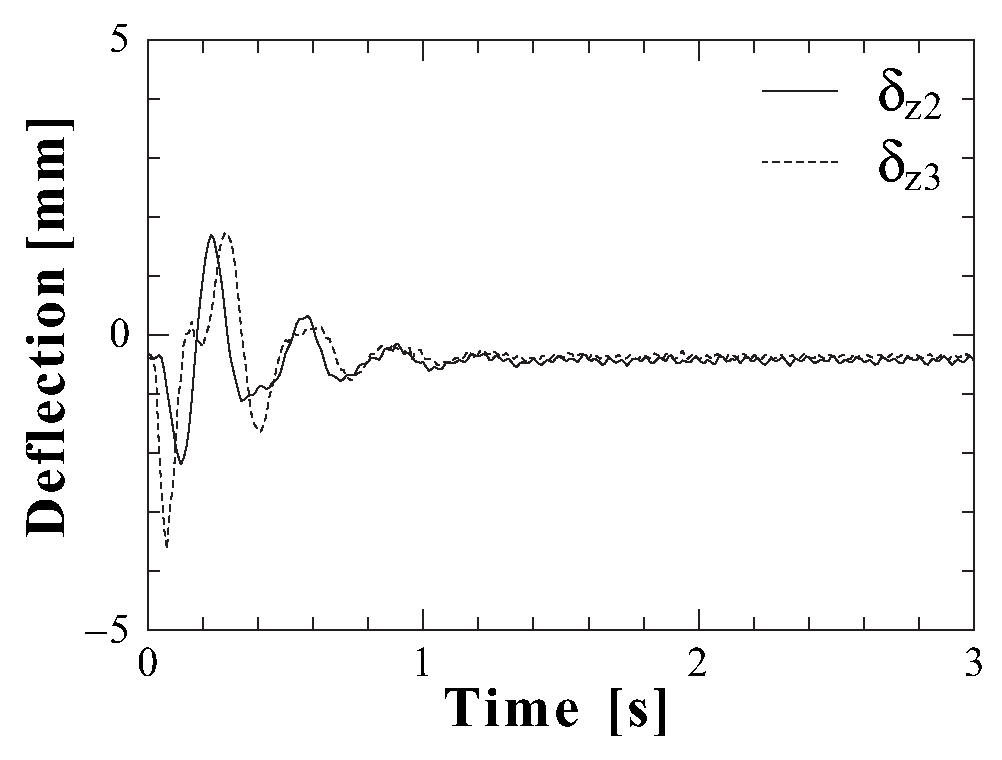
\includegraphics[width=0.8\linewidth]{fig1.eps}
 \caption{A sample figure.  \label{fig:samplefig}}
\end{figure}

図と表は，Fig.~1，Table~1のように番号を振り
（Fig.~\ref{fig:samplefig}\ 参照），図説，図中の説明文は英文で記入してく
ださい．
本文で引用する場合も「Fig.~1に示す」などのようにFig.とTableを使用してく
ださい．

図や表中の文字は小さくなりすぎないよう気をつけてください．
PDF原稿を作成する際，図の画質が劣化しないよう，注意してください．
特にMicrosoft Wordなどで原稿を作成する際，JPEG画像を貼り付けると，一度圧
縮されている画像が再圧縮され画質が劣化するようです．
貼り付ける画像は，画質の良い（圧縮率の低い）画像を用いるか圧縮しない画像
フォーマットを選ぶなど，各自工夫し，最終的なPDFファイルにおいて画質が劣
化しないよう注意してください（300 dpi以上の画質を推奨します）．


\subsection{数式関係}
\verb+eqnarray+ を使うと，等号（とは限りませんが）の両側のスペースが
広くなりすぎるので，この間隔を変更しています．

以下は，\verb+eqnarray+ 環境の使用例です．
\begin{eqnarray}
 \dot{x}(t) & = & A x(t) + B u(t) \\
 y(t) & = & C x(t) + D u(t)
\end{eqnarray}


\subsection{定理環境}
以下は，theorem 環境の使用例です．

\begin{theorem}
ここに定理の内容を記述して下さい．系や補題の場合も同様です．
\end{theorem}
\begin{proof}
ここには定理の証明を記述して下さい．証明の最後には□印がつきま
す．
\end{proof}

定理などの文章は，もともとイタリック書体を使うようになってい
ますが，和文との整合性を考えて，ローマン書体を使うように変更
しています．

\section{参考文献}



文献の引用は本文中に~\cite{web,Conference,Journal}のように書き，
本文の最後にまとめて記述します．次のフォーマットを推奨します．

\begin{enumerate}
  \setlength{\topsep}{0pt}
  \setlength{\partopsep}{0pt}
  \setlength{\itemsep}{0pt}
  \setlength{\parsep}{0pt}
  \setlength{\parskip}{1pt plus 1pt minus 1pt}
	\item[a)] 雑誌論文の場合\\
	$[$番号$]$ 著者：論文題目；雑誌名，Vol.~巻, No.~号, pp.~始ページ--終ページ (発行年)
	\item[b)] 会議論文の場合\\
	$[$番号$]$ 著者：論文題目；会議論文誌名，pp.~始ページ--終ページ (発行年)
	\item[c)] 単行本の場合\\
	$[$番号$]$ 著者：書名，pp.~始ページ--終ページ, 発行所 (発行年)
	\item[c)] Websiteの場合\\
	$[$番号$]$ URL
\end{enumerate}

\begin{thebibliography}{9}
\bibitem{web}
http://www.jjacc.org/

\bibitem{Conference}
自動，制御，自動：
自動制御連合講演会サンプル原稿；
第65回自動制御連合講演会予稿集，pp.~1--4 (2023)

\bibitem{Journal}
T. Jido and J. Jido: Paper title; \textit{Journal Title}, Vol.~1, No.~1, pp.~1--4 (2023)

\bibitem{Book}
H. Seigyo: \textit{Book Title}, pp.~1--4, Publisher (2023)

\end{thebibliography}
\end{document}
% end of template.tex
